\documentclass[tikz,border=12pt]{standalone}
\usepackage[T1]{fontenc}
\usepackage{mathpazo}
\usepackage{amsmath,amssymb}
\usetikzlibrary{arrows.meta, positioning, calc, fit, patterns, decorations.pathreplacing}

\definecolor{stblue}{HTML}{7B97AD}
\definecolor{rwgold}{HTML}{B8995E}
\definecolor{sage}{HTML}{7A9A7E}
\definecolor{dkbrown}{HTML}{3D3530}
\definecolor{wmgray}{HTML}{7B7067}
\definecolor{cream}{HTML}{F9F6F0}
\definecolor{border}{HTML}{D4C9B8}
\definecolor{terracotta}{HTML}{C47A6A}
\definecolor{lavender}{HTML}{907EA0}

\begin{document}
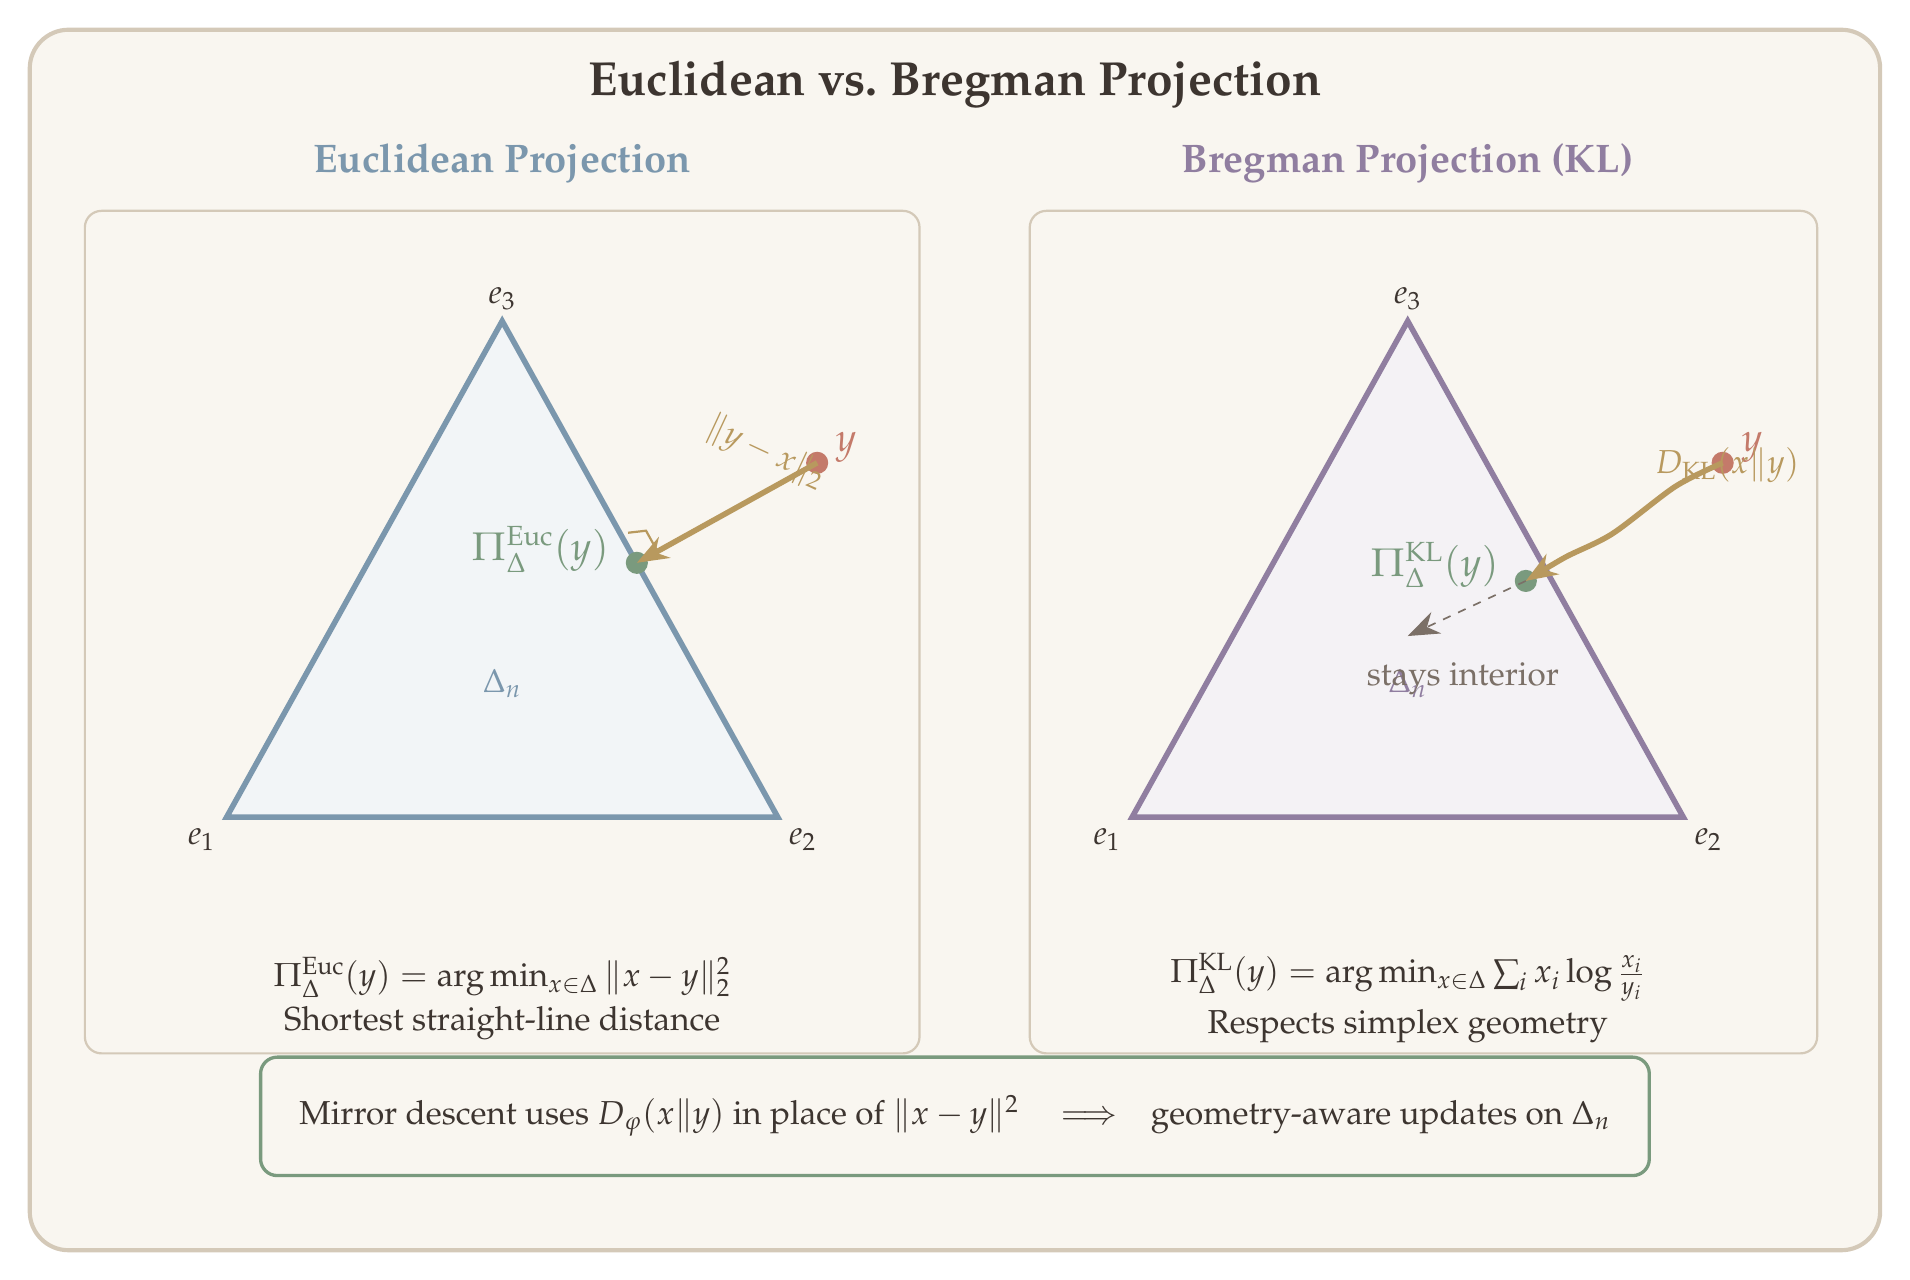
\begin{tikzpicture}[>={Stealth[length=4mm, width=3mm]}, line width=1.5pt]

% Background
\fill[cream, rounded corners=14pt] (-1.5,-5.0) rectangle (22,10.5);
\draw[border, line width=1.5pt, rounded corners=14pt] (-1.5,-5.0) rectangle (22,10.5);

% Title
\node[font=\LARGE\bfseries, text=dkbrown] at (10.25,9.8) {Euclidean vs.\ Bregman Projection};

% =========== LEFT PANEL: Euclidean Projection ===========
\node[font=\Large\bfseries, text=stblue] at (4.5,8.8) {Euclidean Projection};

\draw[border, line width=0.8pt, rounded corners=6pt] (-0.8,-2.5) rectangle (9.8,8.2);

% Simplex as triangle
\coordinate (A1) at (1,0.5);
\coordinate (B1) at (8,0.5);
\coordinate (C1) at (4.5,6.8);

\fill[stblue!10] (A1) -- (B1) -- (C1) -- cycle;
\draw[stblue, line width=2pt] (A1) -- (B1) -- (C1) -- cycle;

% Vertex labels
\node[font=\large, text=dkbrown, below left] at (A1) {$e_1$};
\node[font=\large, text=dkbrown, below right] at (B1) {$e_2$};
\node[font=\large, text=dkbrown, above] at (C1) {$e_3$};

\node[font=\large, text=stblue] at (4.5,2.2) {$\Delta_n$};

% Point outside simplex
\coordinate (P1) at (8.5,5.0);
\fill[terracotta] (P1) circle (4pt);
\node[font=\Large, text=terracotta, right] at (8.6,5.2) {$y$};

% Euclidean projection: orthogonal projection of y=(8.5,5) onto edge B1C1
% B1=(8,0.5), C1=(4.5,6.8), t=0.512 => Proj=(6.21,3.73)
\coordinate (Proj1) at (6.21,3.73);
\fill[sage] (Proj1) circle (4pt);
\node[font=\Large, text=sage, left] at (6.0,3.9) {$\Pi_{\Delta}^{\mathrm{Euc}}(y)$};

% Straight arrow (shortest distance)
\draw[->, rwgold, line width=2pt] (P1) -- (Proj1);

% Right angle marker
\coordinate (M1) at ($(Proj1)!0.3cm!(P1)$);
\coordinate (M1perp) at ($(M1)!0.3cm!90:(P1)$);
\coordinate (M1corner) at ($(M1perp)!0.3cm!(Proj1)$);
\draw[rwgold, line width=0.8pt] (M1) -- (M1perp) -- ($(M1perp)+(M1corner)-(M1)$);

% Distance label
\node[font=\large, text=rwgold, above, rotate=-25] at (7.7,4.8) {$\|y - x\|_2$};

% Caption
\node[font=\large, text=dkbrown, align=center] at (4.5,-1.8)
  {$\Pi_{\Delta}^{\mathrm{Euc}}(y) = \arg\min_{x \in \Delta} \|x - y\|_2^2$\\[2pt]
   Shortest straight-line distance};

% =========== RIGHT PANEL: Bregman Projection ===========
\node[font=\Large\bfseries, text=lavender] at (16,8.8) {Bregman Projection (KL)};

\draw[border, line width=0.8pt, rounded corners=6pt] (11.2,-2.5) rectangle (21.2,8.2);

% Simplex as triangle
\coordinate (A2) at (12.5,0.5);
\coordinate (B2) at (19.5,0.5);
\coordinate (C2) at (16,6.8);

\fill[lavender!10] (A2) -- (B2) -- (C2) -- cycle;
\draw[lavender, line width=2pt] (A2) -- (B2) -- (C2) -- cycle;

% Vertex labels
\node[font=\large, text=dkbrown, below left] at (A2) {$e_1$};
\node[font=\large, text=dkbrown, below right] at (B2) {$e_2$};
\node[font=\large, text=dkbrown, above] at (C2) {$e_3$};

\node[font=\large, text=lavender] at (16,2.2) {$\Delta_n$};

% Same point outside simplex
\coordinate (P2) at (20,5.0);
\fill[terracotta] (P2) circle (4pt);
\node[font=\Large, text=terracotta, right] at (20.1,5.2) {$y$};

% Bregman projection: curved path to simplex (respects geometry)
\coordinate (Proj2) at (17.5,3.5);
\fill[sage] (Proj2) circle (4pt);
\node[font=\Large, text=sage, left] at (17.3,3.7) {$\Pi_{\Delta}^{\mathrm{KL}}(y)$};

% Curved arrow (Bregman path)
\draw[->, rwgold, line width=2pt, smooth]
  plot coordinates {(20,5.0) (19.4,4.7) (18.6,4.1) (18.0,3.8) (17.5,3.5)};

% KL divergence label
\node[font=\large, text=rwgold, above right] at (19,4.6) {$D_{\mathrm{KL}}(x\|y)$};

% Show that projection stays in interior (away from boundary)
\draw[wmgray, line width=0.6pt, dashed, ->] (17.5,3.5) -- (16,2.8);
\node[font=\large, text=wmgray, below] at (16.7,2.6) {stays interior};

% Caption
\node[font=\large, text=dkbrown, align=center] at (16,-1.8)
  {$\Pi_{\Delta}^{\mathrm{KL}}(y) = \arg\min_{x \in \Delta} \sum_i x_i \log\frac{x_i}{y_i}$\\[2pt]
   Respects simplex geometry};

% Bottom comparison
\node[fill=cream, draw=sage, line width=1.2pt, rounded corners=6pt,
      font=\large, text=dkbrown, align=center, inner sep=14pt]
  at (10.25,-3.3) {Mirror descent uses $D_\varphi(x\|y)$ in place of $\|x-y\|^2$
  \quad$\Longrightarrow$\quad geometry-aware updates on $\Delta_n$};

\end{tikzpicture}
\end{document}
